\section{Introduction}
\subsection{Properties of Neurons}
\rem \emph{Neurons} are highly specialized for generating electrical signals in response to chemical and other inputs, and transmitting them to other cells. \emph{Dendrites} receive information inputs from other neurons. \emph{Axons} carry the neuronal output to other cells. The cell body of a neuron is also called the \emph{soma}.
\begin{center}
    \label{fig:1.1}
    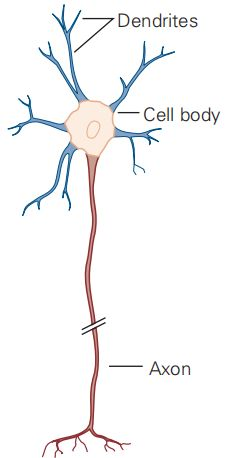
\includegraphics[scale = 0.35]{png/Figure1-1}\\
\end{center}

\rem \emph{Ion channels} control the flow of ions across the cell membrane by opening and closing in response to voltage changes and to both internal and external signals.
\begin{center}
  \label{fig:1.2}
  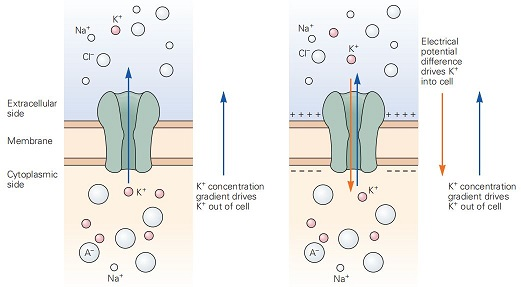
\includegraphics[scale = 0.55]{png/Figure1-2}\\
\end{center}
  
\defn %[Membrane Potential]
The difference in electrical potential between the interior of a neuron and the surrounding extracellular medium is called the \emph{membrane potential}.
\defn
Every cell, including a neuron, maintains a certain difference in the electrical potential on either side of the plasma membrane when the cell is at rest. This is called the \emph{resting membrane potential}.
%The potential difference between two solutions separated by membranes, generally refers to the electrical phenomenon accompanying the life activities of cells, which exists on both side of cells.
\rem Under resting conditions, the potential inside the cell membrane is negative, outside the cell membrane is positive, and the cell is said to be \emph{polarized}. \emph{Ion pumps} located in the cell membrane maintain concentration gradients that support this membrane potential difference.

\defn %[Action Potential]
An \emph{action potential} is the characteristic electrical pulses or, more simply, spikes that can travel down nerve fibers.

\defn %[Hyperpolarization]
Current in the form of positively charged ions flowing out of the cell (or negatively charged ions flowing into the cell) through open channels makes the membrane potential more negative, a process called \emph{hyperpolarization}.

\defn %[Depolarization]
Current flowing into the cell changes the membrane potential to less negative or even positive values. This is called \emph{depolarization}.
\rem If a neuron is depolarized sufficiently to raise the membrane potential above a threshold level, a positive feedback process is initiated, and the neuron generates an action potential.

\defn [Refractory Period]
For a few milliseconds just after an action potential has been fired, it may be virtually impossible to initiate another spike. This is called the \emph{absolute refractory period}. For a longer interval known as the \emph{relative refractory period}, lasting up to tens of milliseconds after a spike, it is more difficult to evoke an action potential.

\rem The absolute refractory period and relative refractory period are two basic phenomena in the process of neural response.

\rem Action potentials are the only form of membrane potential fluctuation that can propagate over large distances. They are regenerated actively along axon processes and can travel rapidly over large distances without attenuation.
\subsection{Recording Neuronal Responses}

\begin{rul}
  Membrane potentials are measured intracellularly by connecting a hollow glass electrode filled with a conducting electrolyte to a neuron, and comparing the potential it records with that of a reference electrode placed in the extracellular medium.
  \begin{enumerate}[(i)]
  \item \emph{Intracellular recordings} are made either with sharp electrodes inserted through the membrane into the cell, or patch electrodes that have broader tips and are sealed tightly to the surface of the membrane. After the patch electrode seals, the membrane beneath its tip is either broken or perforated, providing electrical contact with the interior of the cell.
  \item \emph{Extracellular recordings} placed an electrode near a neuron but it does not penetrate the cell membrane.
  \end{enumerate}
\end{rul}

\begin{rem}
  Extracellular recordings can reveal the action potentials fired by a neuron, but not its subthreshold membrane potentials, and are typically used for in vivo experiments. Intracellular recording is more
commonly used for in vitro preparations.
\end{rem}

\begin{exm}
  Three simulated recordings from a neuron.
  \begin{center}
    \label{fig:1.3}
    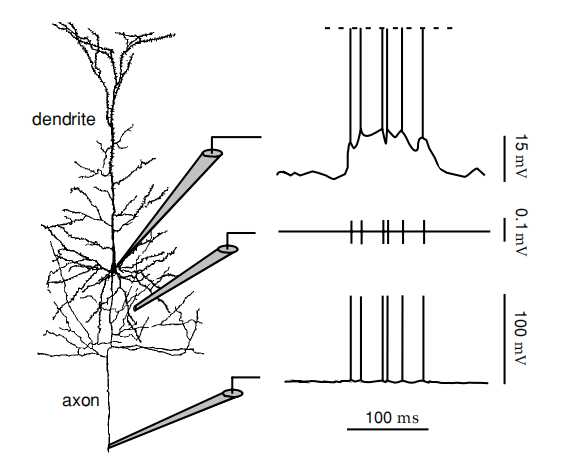
\includegraphics[scale = 0.35]{png/Figure1-3}\\
  \end{center}
  (i) The top trace represents a recording from an intracellular electrode connected to the soma of the neuron. The height of the action potentials has been clipped to show the subthreshold membrane potential more clearly. (ii) The middle trace is a simulated extracellular recording. (iii) The bottom trace represents a recording from an intracellular electrode connected to the axon some distance away from the soma.
\end{exm}



\subsection{From Stimulus to Response}
\rem  Neurons typically respond by producing complex spike sequences that reflect both the intrinsic dynamics of the neuron and the temporal characteristics of the stimulus.
\defn \emph{Neural encoding} refers to the map from stimulus to response.
\exm We can catalog how neurons respond to a wide variety of stimuli, and then construct models that attempt to predict responses to other stimuli.
\defn \emph{Neural decoding} refers to the reverse map, from response to stimulus.
\rem The complexity and trial-to-trial variability of action potential sequences make it unlikely that we can describe and predict the timing of each spike deterministically. Instead, we seek a model that can account for the probabilities that different spike sequences are evoked by a specific stimulus.


%%% Local Variables:
%%% mode: latex
%%% TeX-master: t
%%% End:
